\documentclass{standalone}
\usepackage{tikz}
\begin{document}
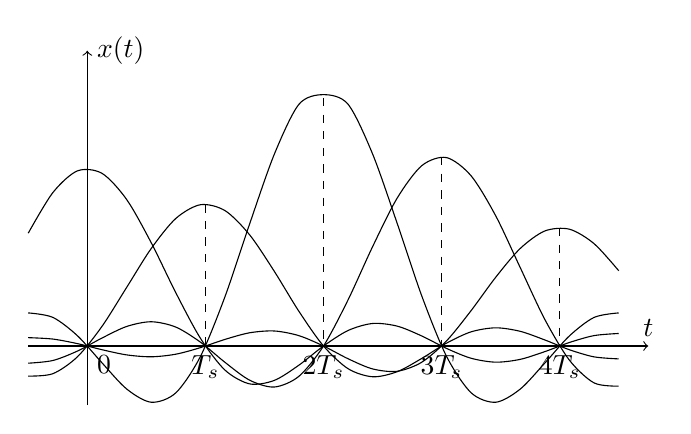
\begin{tikzpicture}[scale=3]
    \draw[->](-0.25,0)--(2.375,0)node[above]{$t$};
    \draw[->](0,-0.25)--(0,1.25)node[right]{$x(t)$};
    \draw[smooth, domain=-0.25:2.25]plot(\x,{0.75*sin(2*pi*\x r)/(2*pi*\x)});
    \draw[smooth, domain=-0.25:2.25]plot(\x,{0.6*sin(2*pi*(\x-0.5) r)/(2*pi*(\x-0.5))});
    \draw[smooth, domain=-0.25:2.25]plot(\x,{1.1*sin(2*pi*(\x-1) r)/(2*pi*(\x-1))});
    \draw[smooth, domain=-0.25:2.25]plot(\x,{0.8*sin(2*pi*(\x-1.5) r)/(2*pi*(\x-1.5))});
    \draw[smooth, domain=-0.25:2.25]plot(\x,{0.5*sin(2*pi*(\x-2) r)/(2*pi*(\x-2))});
    \node[below right]at(0,0){$0$};
    \draw[dashed](0.5,0.6)--(0.5,0)node[below]{$T_s$};
    \draw[dashed](1,1.05)--(1,0)node[below]{$2T_s$};
    \draw[dashed](1.5,0.8)--(1.5,0)node[below]{$3T_s$};
    \draw[dashed](2,0.5)--(2,0)node[below]{$4T_s$};
\end{tikzpicture}
\end{document}